\chapter{Entwurf und Design}

\authoredsection{Laura}{Design}
Der visuelle Eindruck und die Benutzerfreundlichkeit einer Lernplattform spielen eine entscheidende Rolle in Bezug auf die Motivation der Lernenden. Die Schaffung einer benutzerfreundlichen und ansprechenden Lernumgebung ist ein zentraler Aspekt, der in diesem Kapitel umfassend betrachtet wird.
Die bereits ermittelten Anforderungen bilden die Basis für die Gestaltung der Prototypen, die im Verlauf dieses Kapitels behandelt werden.
Anschließend wird eine Auswahl von besonders wichtigen Ansichten der Plattform vorgestellt zusammen mit vorgenommenen Veränderungen und Designentscheidungen im Verlauf der Entwicklung.

\subsection{GUI-Prototyping}
Mithilfe der erstellten Anforderungen und User Stories werden die Prototypen für das Graphical User Interface (GUI) erstellt. Diese dienen als gute Grundlage und Ansatzpunkt für die spätere Umsetzung und Entwicklung. 
So kann bereits ein Überblick über den Umfang der Plattform und einem einheitlichen Design erschaffen werden. 

\subsubsection{Mock-Ups}
Die Mock-Ups wurden mithilfe von Wireframe-Werkzeugen und den Vorlagen von Miro entwickelt. Miro, als Online-Kollaborationsplattform, unterstützt das gemeinsame Planen, die Informationszusammenstellung und die Entwicklung dieses Projekts.

Für die Mock-Ups wird zunächst das grundlegende Design und Layout festgelegt. Dies soll dazu führen, dass eine konsistente Gestaltung sichergestellt wird. Basierend auf dieser Basis werden weitere Ansichten im gleichen Stil erstellt, wodurch eine Einheitlichkeit und Kohärenz zwischen den Ansichten gewährleistet wird. Das in Abbildung \ref{fig:Layout Mock-Up} dargestellte Layout bildet hierbei den Ausgangspunkt.

\begin{figure}
    \centering
    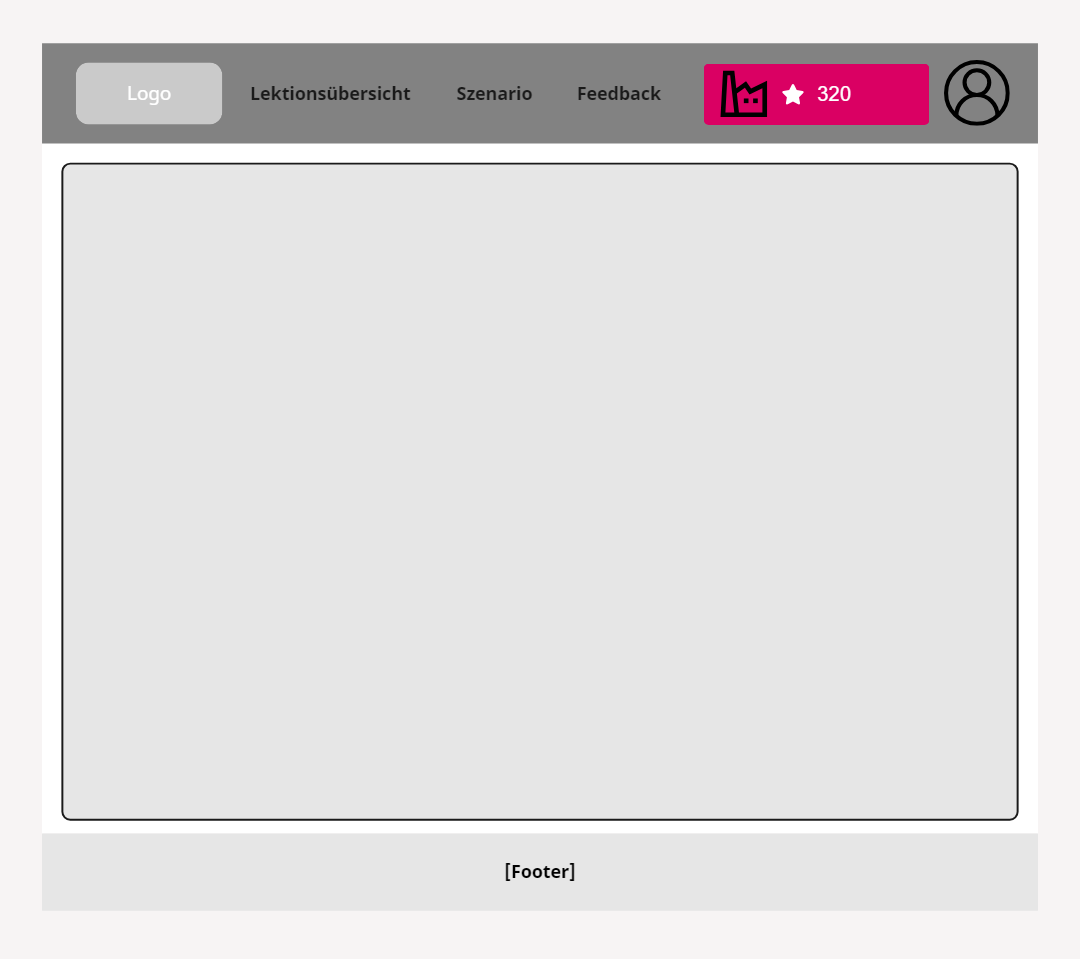
\includegraphics[width=1.0\textwidth]{assets/screenshots/mockups/Layout-MockUp.png}
    \caption{Layout des Mock-Ups}
    \label{fig:Layout Mock-Up}
\end{figure}

Oben ist die Navigationsleiste erkenntlich, welche das Logo der Lernplattform, wichtigen Reiter für diverse Übungsmöglichkeiten, wie die Lektionen und Szenarien und eine Option Feedback abzusenden. Hierdurch soll der Zugang zur nächsten Übung oder Lektion einfach und erkenntlich gemacht werden.
Des Weiteren werden die Punkte für das ausgewählte Unternehmen angezeigt. Diese Anzeige betont nicht nur den Fortschritt des Lernenden, sondern dient auch der Anregung, weitere Punkte zu sammeln. Der Lernende kann sich dadurch kompetent und bestätigt in seiner Lernerfahrung fühlen. Das Erleben von Kompetenz als psychologisches Grundbedürfnis kann somit die Motivation steigern, mehr zu lernen und dadurch mehr Punkte zu sammeln.\footcite[vgl.][S.516-517]{BolognaDigital}
Ein Nutzer-Icon für das Profil des Lernenden oder Lehrenden ist ebenfalls vorhanden, um persönliche Daten anzuzeigen. 
Der verbleibende Platz in den folgenden Mock-Ups wird individuell mit den benötigten Elementen und Informationen für die verschiedenen Ansichten gefüllt.

\subsection{Wichtige Ansichten}

\subsubsection{Startseite}

Die Startseite wird in Abbildung \ref{fig:Startseite Mock-Up} dargestellt. Diese ist für alle zugänglich und bietet den Einstieg in die Plattform, wenn man sich noch nicht registriert oder angemeldet hat. 
Von hieraus wird die Möglichkeit angeboten sich anzumelden oder sich einen allgemeinen Überblick über die Lernplattform zu verschaffen.

\begin{figure}[H]
    \centering
    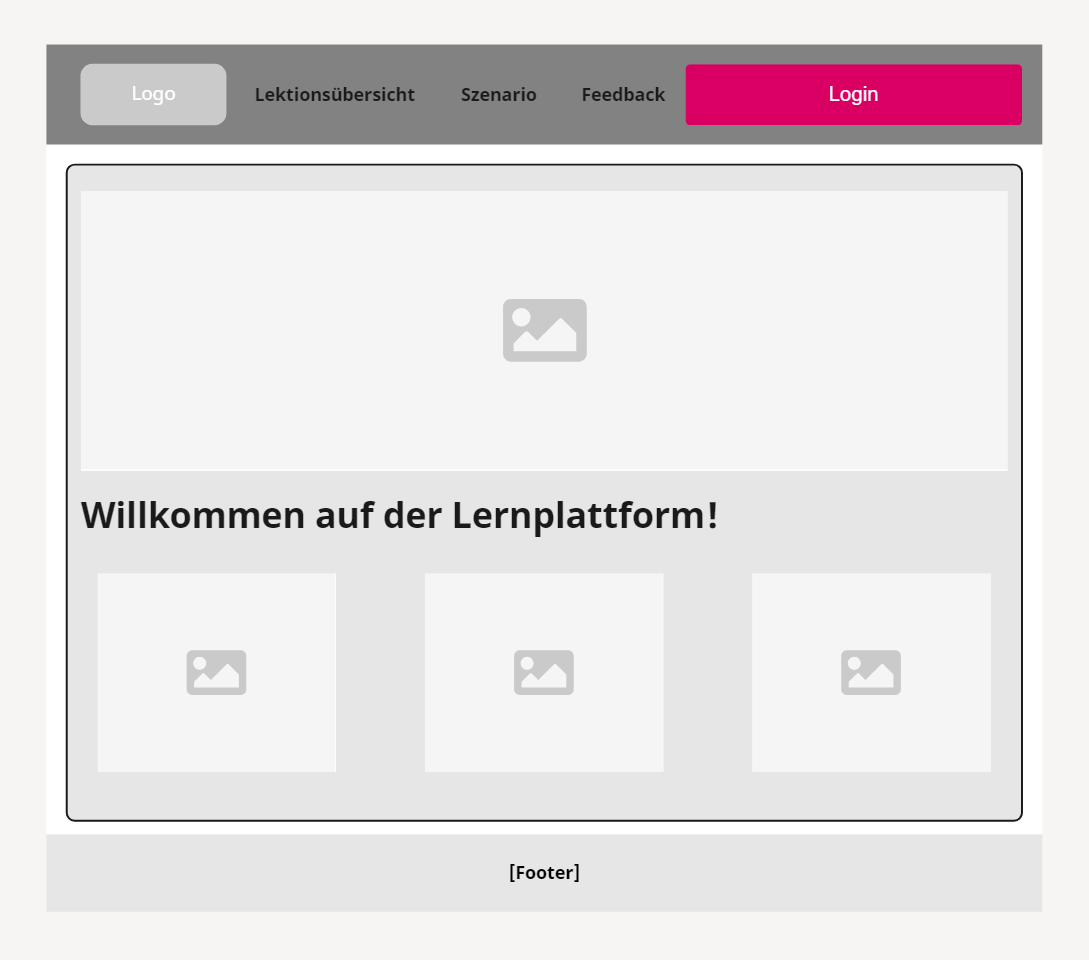
\includegraphics[width=1.0\textwidth]{assets/screenshots/mockups/Homepage-MockUp.png}
    \caption{Startseite}
    \label{fig:Startseite Mock-Up}
\end{figure}


\subsubsection{Anmeldung und Registrierung}

In den nächsten Abbildungen \ref{fig:Anmeldung Mock-Up} und \ref{fig:Registrierung Mock-Up} werden die Ansichten zur Anmeldung und Registrierung dargestellt.
Bei der Registrierung wird, wie in den Anforderungen und den Akzeptanzkriterien definiert, ein Benutzername, eine E-Mail Adresse und ein Passwort benötigt. 
Die Anmeldung selbst erfolgt über die E-Mail und dem Passwort. Weiterhin ist es möglich, das Passwort zurücksetzen zu lassen, falls man es vergessen haben sollte. 
Die Anmeldung sollte möglichst leicht für neue Nutzer zugänglich sein. Dementsprechend wurde die Login Schaltfläche hervorgehoben und ersichtlich für alle nicht angemeldeten Nutzer platziert.
Auch die Registrierung sollte auffindbar sein, indem man vom Login Bereich zur Registrierung wechseln kann.

\begin{figure}[H]
    \centering
    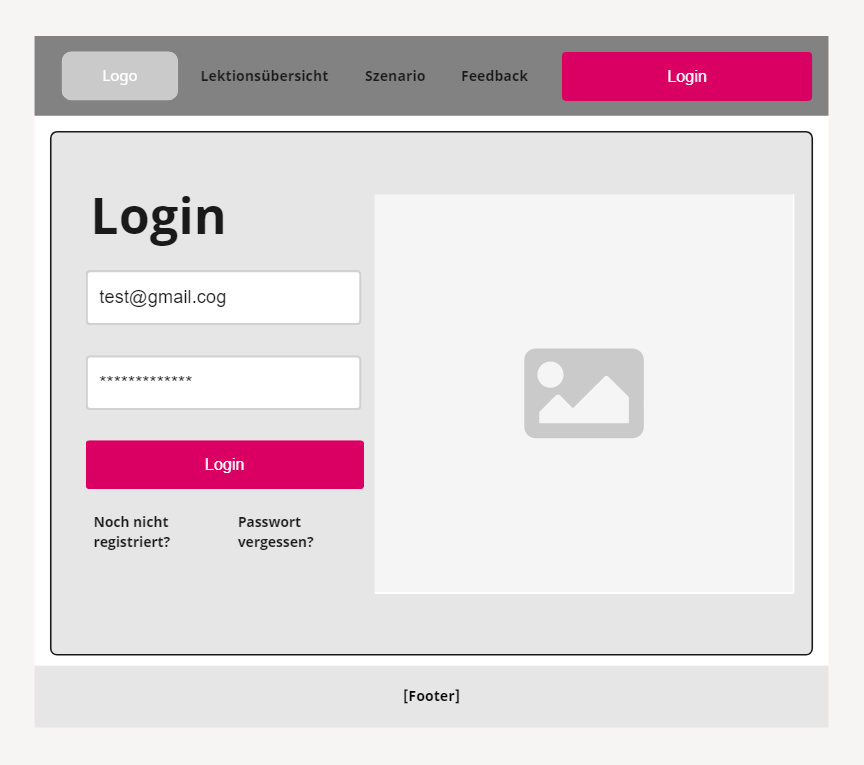
\includegraphics[width=1.0\textwidth]{assets/screenshots/mockups/LogIn-MockUp.png}
    \caption{Anmeldung}
    \label{fig:Anmeldung Mock-Up}
\end{figure}

\begin{figure}[H]
    \centering
    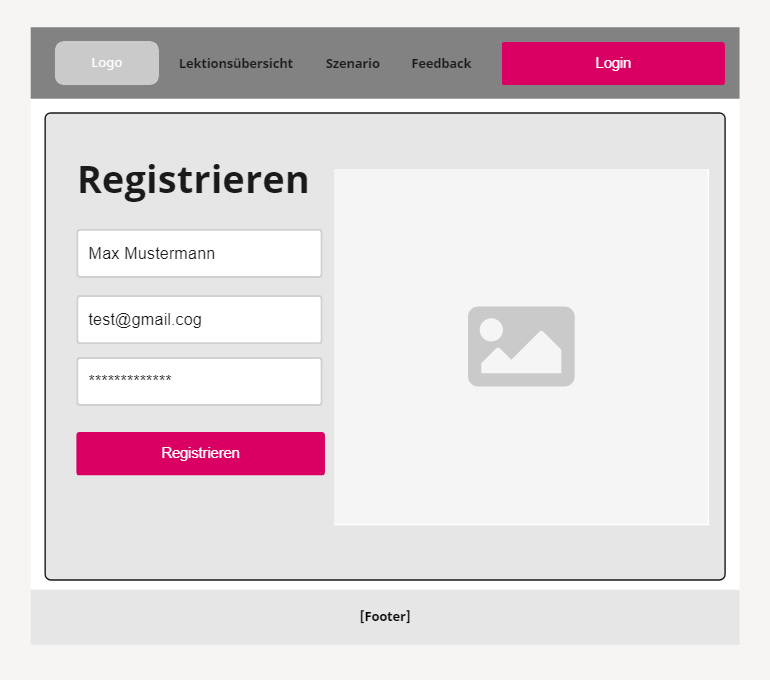
\includegraphics[width=1.0\textwidth]{assets/screenshots/mockups/Register-MockUp.png}
    \caption{Registrierung}
    \label{fig:Registrierung Mock-Up}
\end{figure}

\subsubsection{Profil}

Abbildung \ref{fig:Profil Mock-Up} zeigt die Profilseite des aktuell angemeldeten Nutzers an. Hier sind persönliche Daten, wie Benutzername, E-Mail und das Passwort einsehbar und änderbar. Damit ist eine weitere Anforderung berücksichtigt worden. 
Der aktuelle Fortschritt bezüglich des vom Nutzer ausgewählten Unternehmens wird ebenfalls angezeigt.

\begin{figure}[H]
    \centering
    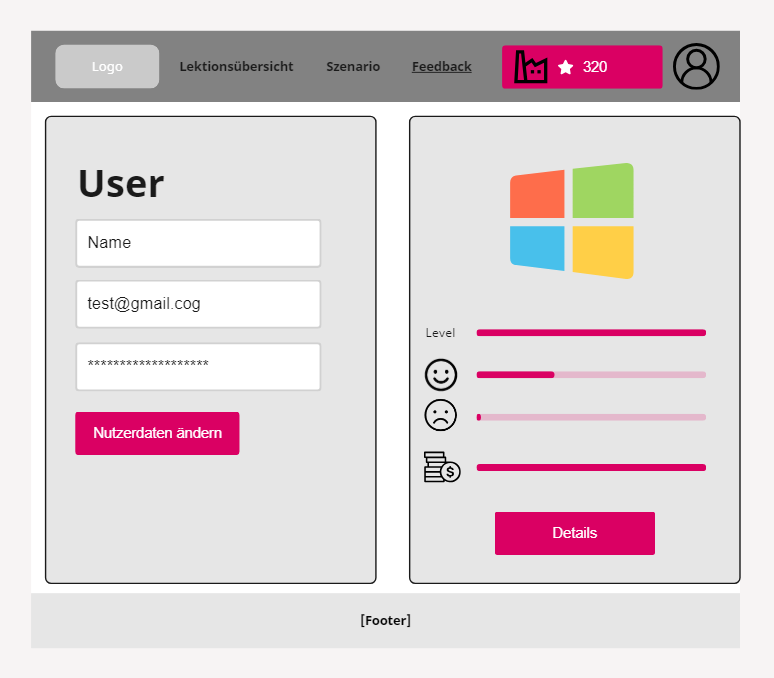
\includegraphics[width=1.0\textwidth]{assets/screenshots/mockups/Profil-MockUp.png}
    \caption{Profil}
    \label{fig:Profil Mock-Up}
\end{figure}

\subsubsection{Hochladen eines Kataloges}

Das Hochladen eines Katalogs stellt eine zentrale Funktion auf der Lernplattform dar. Der Ablauf dieses Vorgangs wird in Abbildung \ref{fig:Katalog_Hochladen} veranschaulicht.
Ein dafür vorgesehenes Feld ermöglicht das einfache Ziehen und Ablegen (Drag and Drop) von Katalogen aus dem Dateisystem. 
Der Name des hochzuladenden Katalogs wird dabei im Feld angezeigt, um eine klare Identifizierung der ausgewählten Datei zu gewährleisten.
Zusätzlich steht unter dem Feld ein Button bereit, der die Auswahl eines Katalogs ermöglicht und den abschließenden Hochladevorgang initiiert. 
Es ist wichtig zu betonen, dass diese Funktion nur für Lehrende oder Administratoren zur Verfügung steht. Dies wird durch die Rolle neben dem Profil in der Navigationsleiste verdeutlicht. 
 
\begin{figure}[H]
    \centering
    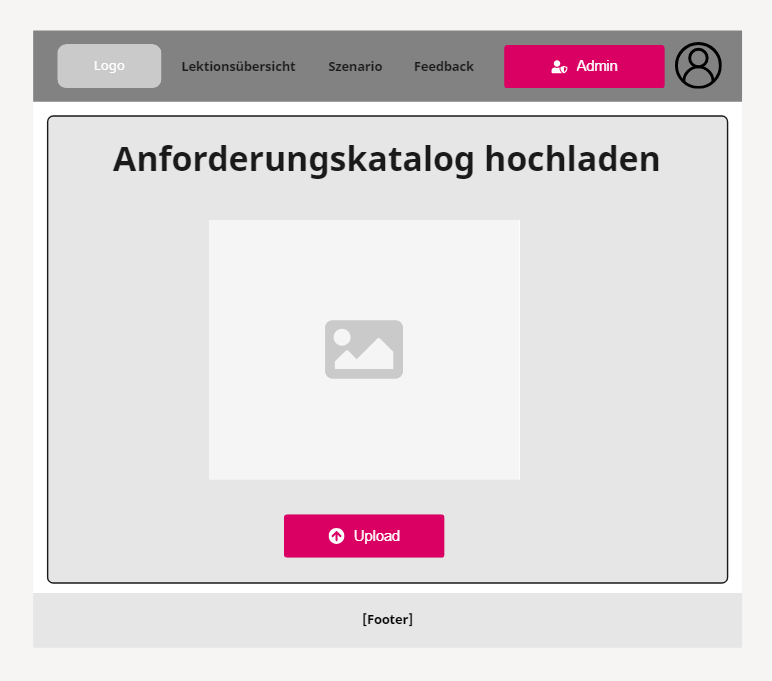
\includegraphics[width=1.0\textwidth]{assets/screenshots/mockups/KatalogUpload-MockUp.png}
    \caption{Hochladen eines Kataloges}
    \label{fig:Katalog_Hochladen}
\end{figure}

\subsubsection{Lektionen und Aufgaben}

Die Ansichten für die Lektionen und Aufgaben gehören unter anderem zu den wichtigsten Ansichten. Diese sollen eine effektive Möglichkeit darbieten, einen Überblick über die Aufgaben zu erhalten. Es ist von besonderer Bedeutung, dass die Aufgaben klar verständlich sind und Interaktionen fördern. 

Innerhalb der Mock-Ups werden zwei zentrale Aufgabenformate unterschieden: die Software-Erprobung und die Software-Auswahl. 
Hierdurch werden verschiedene Lernziele verfolgt. Einmal die Erprobung einer Software, wie durch das Recherchieren von wichtigen Informationen oder dem eigenständigen Testen außerhalb der Lernplattform. Auf diese Weise soll der Lernende lernen, wie eine Software erprobt und ein Anforderungskatalog sinnvoll ausgefüllt wird. Das zweite Ziel beschreibt, in der Lage zu sein, eine Software mithilfe eines Anforderungskataloges und ihren Qualifizierungen zu evaluieren und zu bewerten oder mit anderer Software zu vergleichen. Dabei steht im Fokus, welche Software den vom Unternehmen gewünschten Anforderungen am besten gerecht wird.

In der folgenden Abbildung \ref{fig:Software-Erprobung-1} wird eine Möglichkeit zur Erprobung und Evaluierung einer Software präsentiert.
Die Lektion ist mit einem klaren Titel und einer Beschreibung versehen. Daran schließen sich verschiedene Aufgabentypen an, jeweils mit einem Titel und einer Fragestellung.
Eine interaktive Tabelle repräsentiert den Anforderungskatalog
Sie ist mit den Daten gefüllt, die aus dem Format der hochzuladenen Kataloge bekannt sind. 
Diese Tabelle lässt sich dynamisch ausfüllen, während die Software außerhalb der Plattform erprobt wird.
Dadurch soll ermittelt werden, welche Anforderungen mit welcher Qualifizierung erfüllt werden.
Darüber hinaus ist es möglich, Kommentare mit Begründungen zu den einzelnen Qualifikationen abzugeben.

\begin{figure}[H]
    \centering
    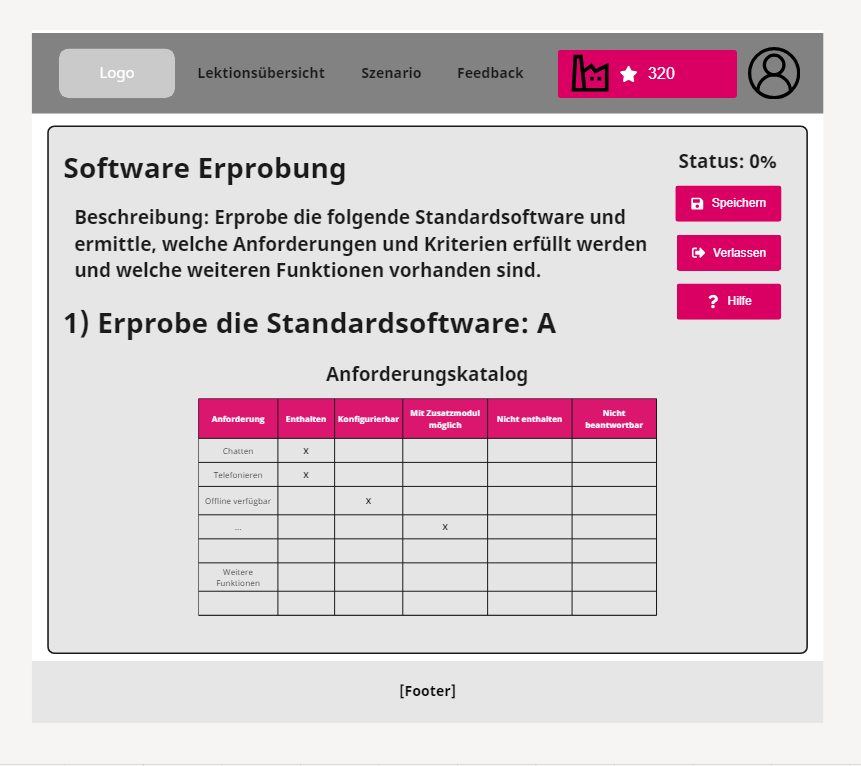
\includegraphics[width=1.0\textwidth]{assets/screenshots/mockups/Software-Erprobung-1.png}
    \caption{Software Erprobung}
    \label{fig:Software-Erprobung-1}
\end{figure}

Des weiteren ist erkenntlich, dass eine Statusanzeige vorhanden ist, welchen den aktuellen Fortschritt der Lektion vermittelt. Diese Anzeige ermöglicht es dem Lernenden, einen klaren Überblick darüber zu erhalten, wie weit er bereits in der Lektion vorangeschritten ist.
Weitere wichtige Anforderungen, wie das Speichern des aktuellen Standes und das spätere Zurückkehren zur Lektion, wurden ebenfalls berücksichtigt. Dies wurde mithilfe von Buttons dargestellt, die das Speichern des Fortschritts ermöglichen. Weiterhin kann die Lektion verlassen werden, so dass man später zu dieser zurückkehren kann, um weiterzuarbeiten. 
Dadurch wird auch ein didaktisches Prinzip erfüllt, das besagt, dass der Lernende Flexibilität erlangt in der Möglichkeit, wann und wo dieser üben möchte.\footcite[Vgl.][S.2]{Minkovska.2016}{}{}
Falls der Lernende Verständnisprobleme bezüglich der Aufgabenbearbeitung hat, gibt es auch eine Hilfe-Option. 

In der nächsten Abbildung \ref{fig:Software-Erprobung-2} wird die Erprobung der Software weitergeführt. Hier wird eine Drag and Drop Aufgabe dargestellt. Man kann die vorgegebenen Funktionen der Software in den passenden Bereich ziehen und ablegen, je nachdem ob die Funktion vorhanden ist oder nicht. 
Diese Aufgabe zielt darauf ab, die Interaktion durch bewegbare Elemente zu erhöhen. 

\begin{figure}[H]
    \centering
    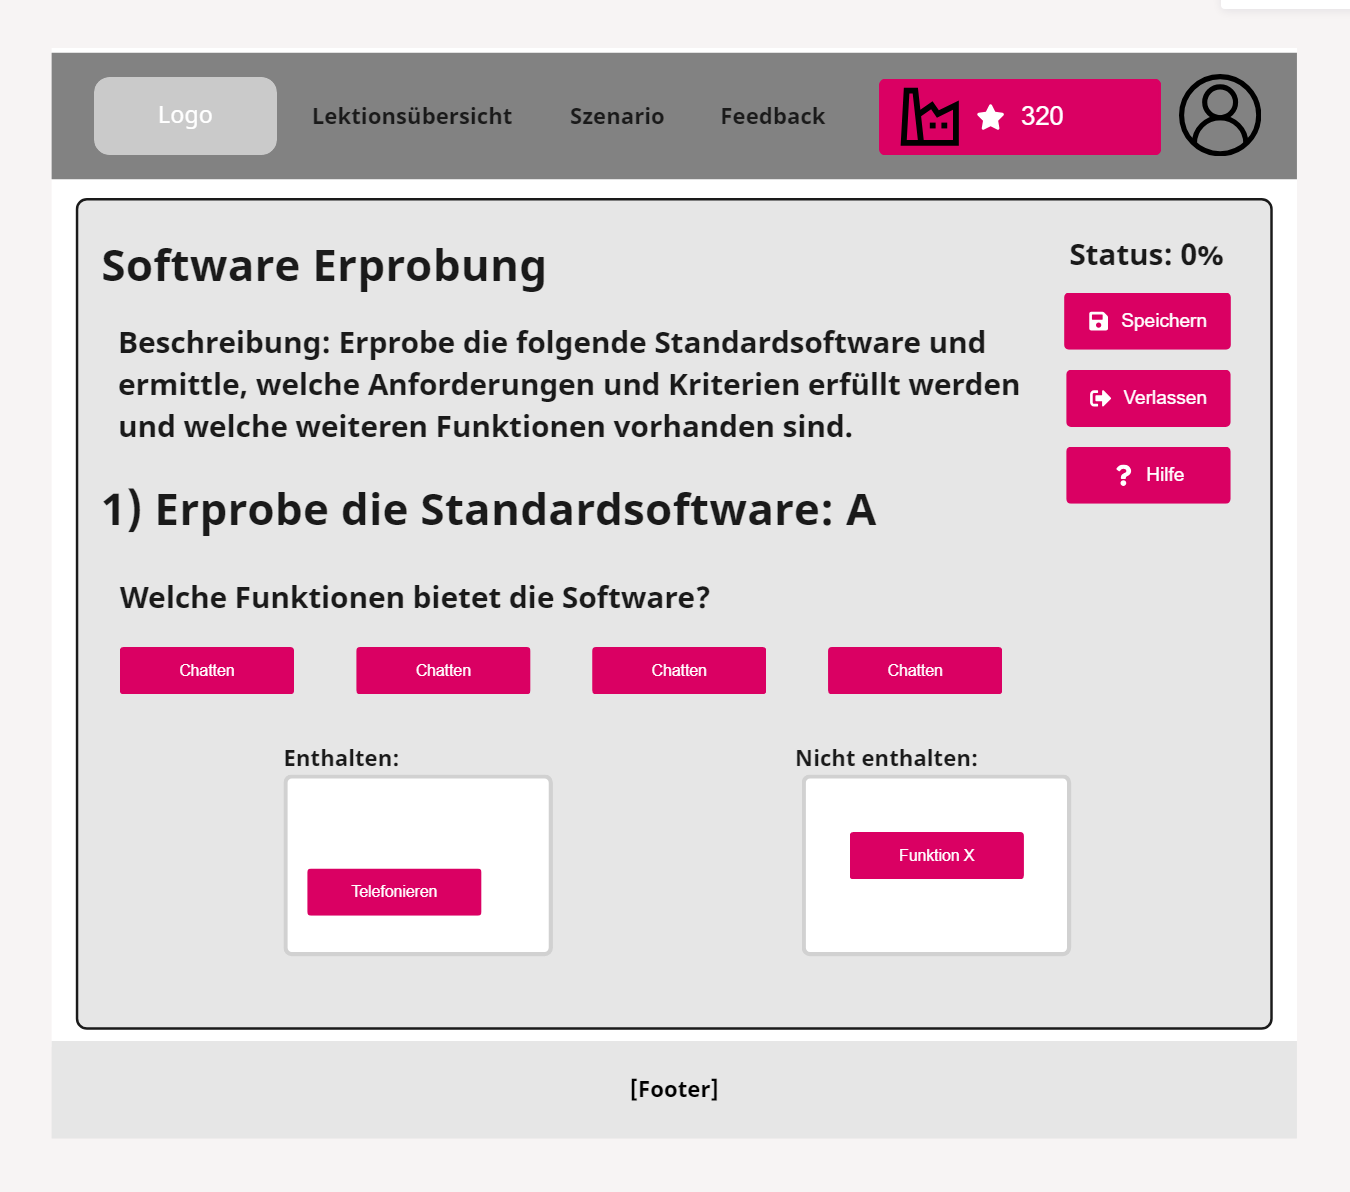
\includegraphics[width=1.0\textwidth]{assets/screenshots/mockups/Software-Erprobung-2.png}
    \caption{Software Erprobung Fortsetzung}
    \label{fig:Software-Erprobung-2}
\end{figure}

In der nächsten Ansicht \ref{fig:Software-Auswahl-1} wird eine andere Art von Aufgabe präsentiert.
Hierbei sollen verschiedene Softwareprodukte miteinander verglichen und hinsichtlich ihrer Eignung bezüglich der definierten Anforderungen und Funktionen bewertet werden. 
Ein bereits ausgefüllter Anforderungskatalog mit definierten Anforderungen und Qualifizierungen dient als Grundlage für diese Aufgabe.

Weiterhin kann der Lernende sich persönliche Notizen zu den Aufgaben oder zum Beispiel zu der Eignungsfähigkeit der Software machen. Die Notizen fließen nicht in die Bewertung ein, sondern dienen als unterstützende Hilfestellung. 

\begin{figure}[H]
    \centering
    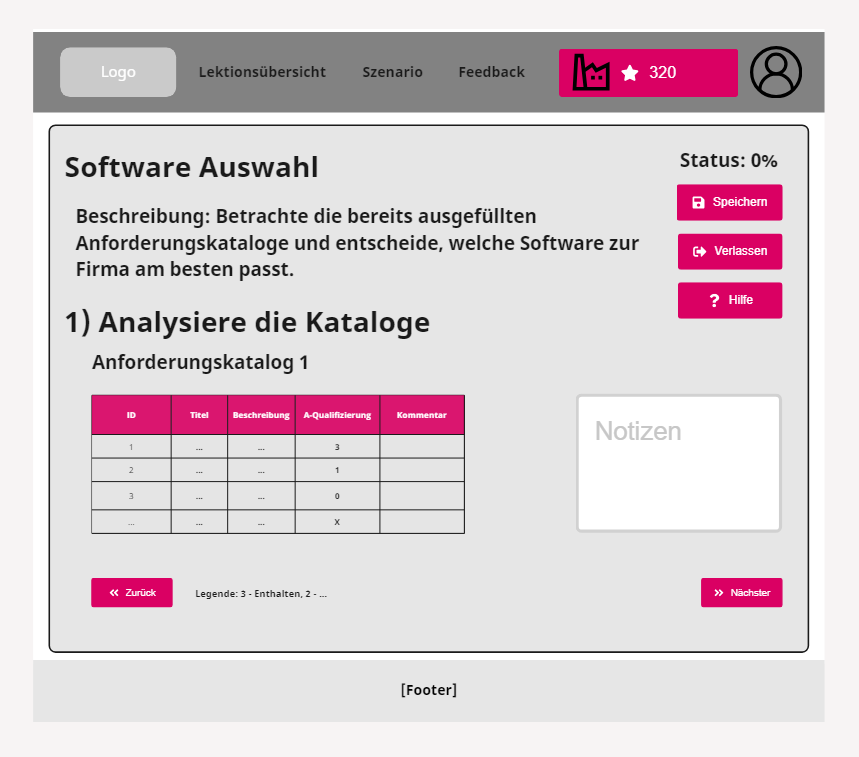
\includegraphics[width=1.0\textwidth]{assets/screenshots/mockups/Software-Auswahl-1.png}
    \caption{Software Auswahl}
    \label{fig:Software-Auswahl-1}
\end{figure}

Die Lektion wird in der nächsten Abbildung \ref{fig:Software-Auswahl-2} fortgeführt. Hier gibt es eine Multiple Choice Frage, wo die Aussagen nach Richtig oder Falsch bewertet werden sollen. Auch hier können die zuvor erstellten Notizen zu den zu vergleichenden Softwareprodukten angezeigt oder verändert werden.

\begin{figure}[H]
    \centering
    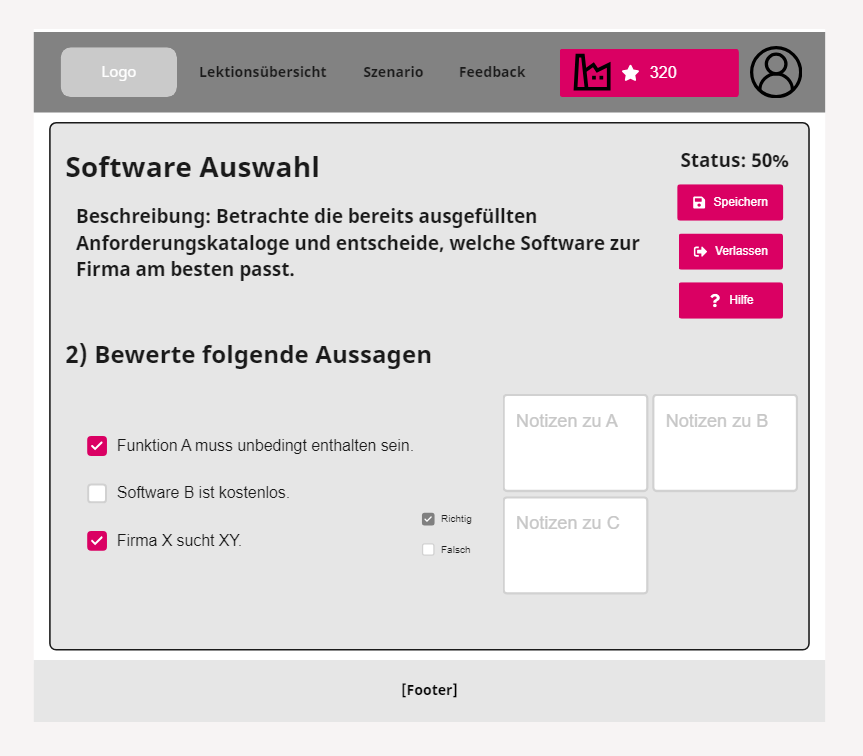
\includegraphics[width=1.0\textwidth]{assets/screenshots/mockups/Software-Auswahl-2.png}
    \caption{Software Auswahl Fortsetzung}
    \label{fig:Software-Auswahl-2}
\end{figure}

Im nächsten der Teil der Aufgabe in Abbildung \ref{fig:Software-Auswahl-3} wird eine Sortieraufgabe angezeigt. Hierfür wird erneut die Drag and Drop Funktion verwendet. Die zu vergleichenden Softwareprodukte sollen nun in eine vom Lernenden gewählte Reihenfolge sortiert werden.  Das Kriterium zur Sortierung ist ihre Eignung bezüglich der Anforderungen, Funktionen und Qualifizierungen. 
Es soll anschließend also eine Reihenfolge von der am besten geeigneten Software, welche mit einer Krone markiert ist, bis hin zur am wenigsten geeigneten Software entstehen.
Auch in dieser Aufgabe werden erneut die Notizen zur Hilfestellung angezeigt, um die Produkte zu evaluieren. 

\begin{figure}[H]
    \centering
    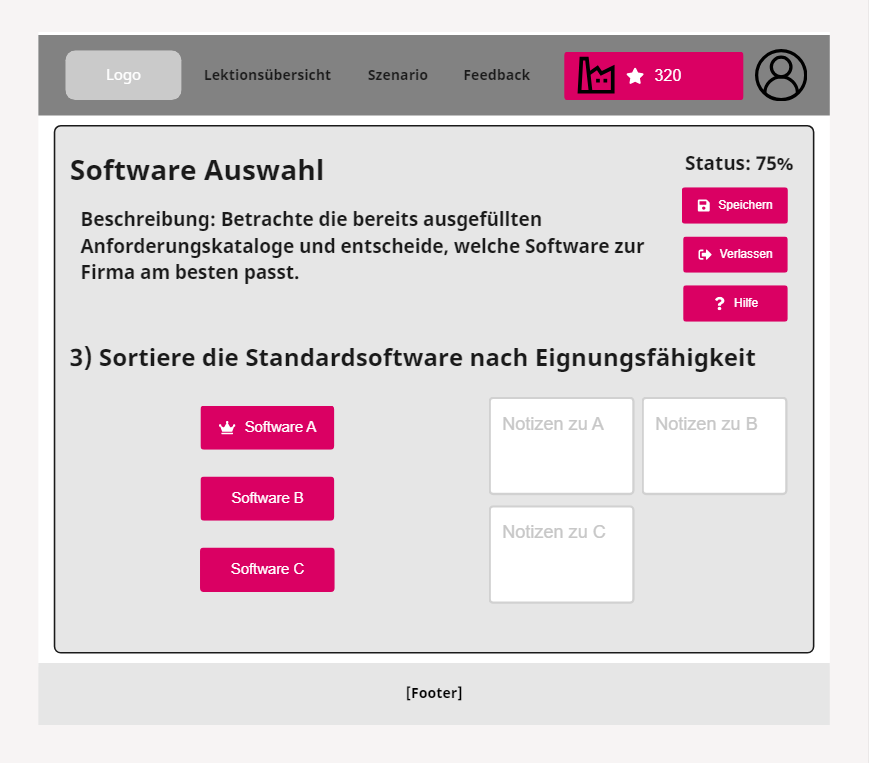
\includegraphics[width=1.0\textwidth]{assets/screenshots/mockups/Software-Auswahl-3.png}
    \caption{Software Auswahl Fortsetzung 2}
    \label{fig:Software-Auswahl-3}
\end{figure}

\subsection{Usability und UX im finalen GUI}

Im Verlauf der Implementierung und Gestaltung des GUIs der Lernplattform hat sich das Layout mehrmals verändert. Einige deutlichen Änderungen und Anpassungen und die Gedanken dahinter werden in diesem Abschnitt einmal vorgestellt. Die Usability und User Experience (UX) wird zudem auch genauer betrachtet.

\subsubsection{Startseite}

Einige klare Unterschiede finden sich bereits in dem Layout in Abbildung \ref{fig:mainpage_gui}. Nicht benötigte Elemente wurden entfernt, so dass der Hauptinhalt im Zentrum steht. Im Vergleich zur Ansicht in \ref{fig:Layout Mock-Up} ist die Navigationsleiste nun nicht mehr konstant oben am Bildschirm platziert, sondern in einer dynamischen Seitenleiste angebracht. Diese lässt sich schließen und öffnen bei Bedarf. Dadurch soll der komplette Platz des Bildschirms möglichst gut ausgenutzt werden, so dass die Inhalte klar und uneingeengt dargestellt werden. Dadurch soll die UX verbessert werden.
Vor allem in Lektionen wird dies von Bedeutung sein, da ein überfüllter Bildschirm für Überforderung und Demotivation sorgen kann. Außerdem gibt es so weniger Ablenkungsmöglichkeiten beim Bearbeiten von Aufgaben.

\begin{figure}[H]
    \centering
    
\includegraphics[width=1.0\textwidth]{assets/screenshots/finale_gui/Hauptseite.png}
    \caption{Hauptseite der Lernplattform}
    \label{fig:mainpage_gui}
\end{figure}

In der frühen Implementierungsphase der Navigation gab es auch bereits einige Schwierigkeiten. Die Navigationsleiste war unübersichtlich und irritierend, denn es gab widersprüchliche oder zu ähnliche Navigationspunkte, so dass man nicht direkt zum Ziel gelangte. Dies kann die UX und Nutzerfreundlichkeit erheblich einschränken. Hier hilft unter anderem der Einsatz von Icons. Diese sollen die Verständlichkeit und Zurechtfindung auf der Plattform unterstützen. So kann man beim Navigieren nicht nur nach Text, sondern auch nach Icons Ausschau halten. 

Die Farbauswahl hat sich ebenfalls deutlich verändert. Es wird ein modernes und ansprechendes Design angestrebt. Die Farben sollen die Plattform und ihre Lektionen interessanter auf den Lernenden und Lehrenden wirken lassen.

Weiterhin ist ein Wechsel zwischen einem hellen und dunklen Thema möglich. 
Das helle Thema wird in der Grafik \ref{fig:light_theme_gui} dargestellt. Dort ist zudem sichtbar, wie die Hauptseite mit eingeklappter Navigationsleiste aussieht.

\begin{figure}[H]
    \centering
    
\includegraphics[width=1.0\textwidth]{assets/screenshots/finale_gui/Light_Theme.png}
    \caption{Hauptseite der Lernplattform im hellen Thema}
    \label{fig:light_theme_gui}
\end{figure}

\subsubsection{Hochladen eines Kataloges}

Die Ansicht zum Hochladen eines Kataloges hat einige zusätzliche Komponenten erhalten, ist vom Aufbau allerdings dem Mock-Up in \ref{fig:Katalog_Hochladen} größtenteils treu geblieben. Sie wurde jedoch um wichtige Hinweise zum Hochladen ergänzt, um möglichen Schwierigkeiten und Problemen entgegenzuwirken. Außerdem wird hier deutlich zwischen dem Drag and Drop Feld und der Auswahl über das Dateisystem unterschieden. 
Weiterhin gibt es Beispielkataloge zum Herunterladen, welche als Vorlage verwendet werden können, um korrekte Kataloge hochladen zu können. Dadurch soll eine mögliche Frustration der Nutzer bei Unverständnis oder ungültigen Formaten verhindert werden.

\begin{figure}[H]
    \centering
    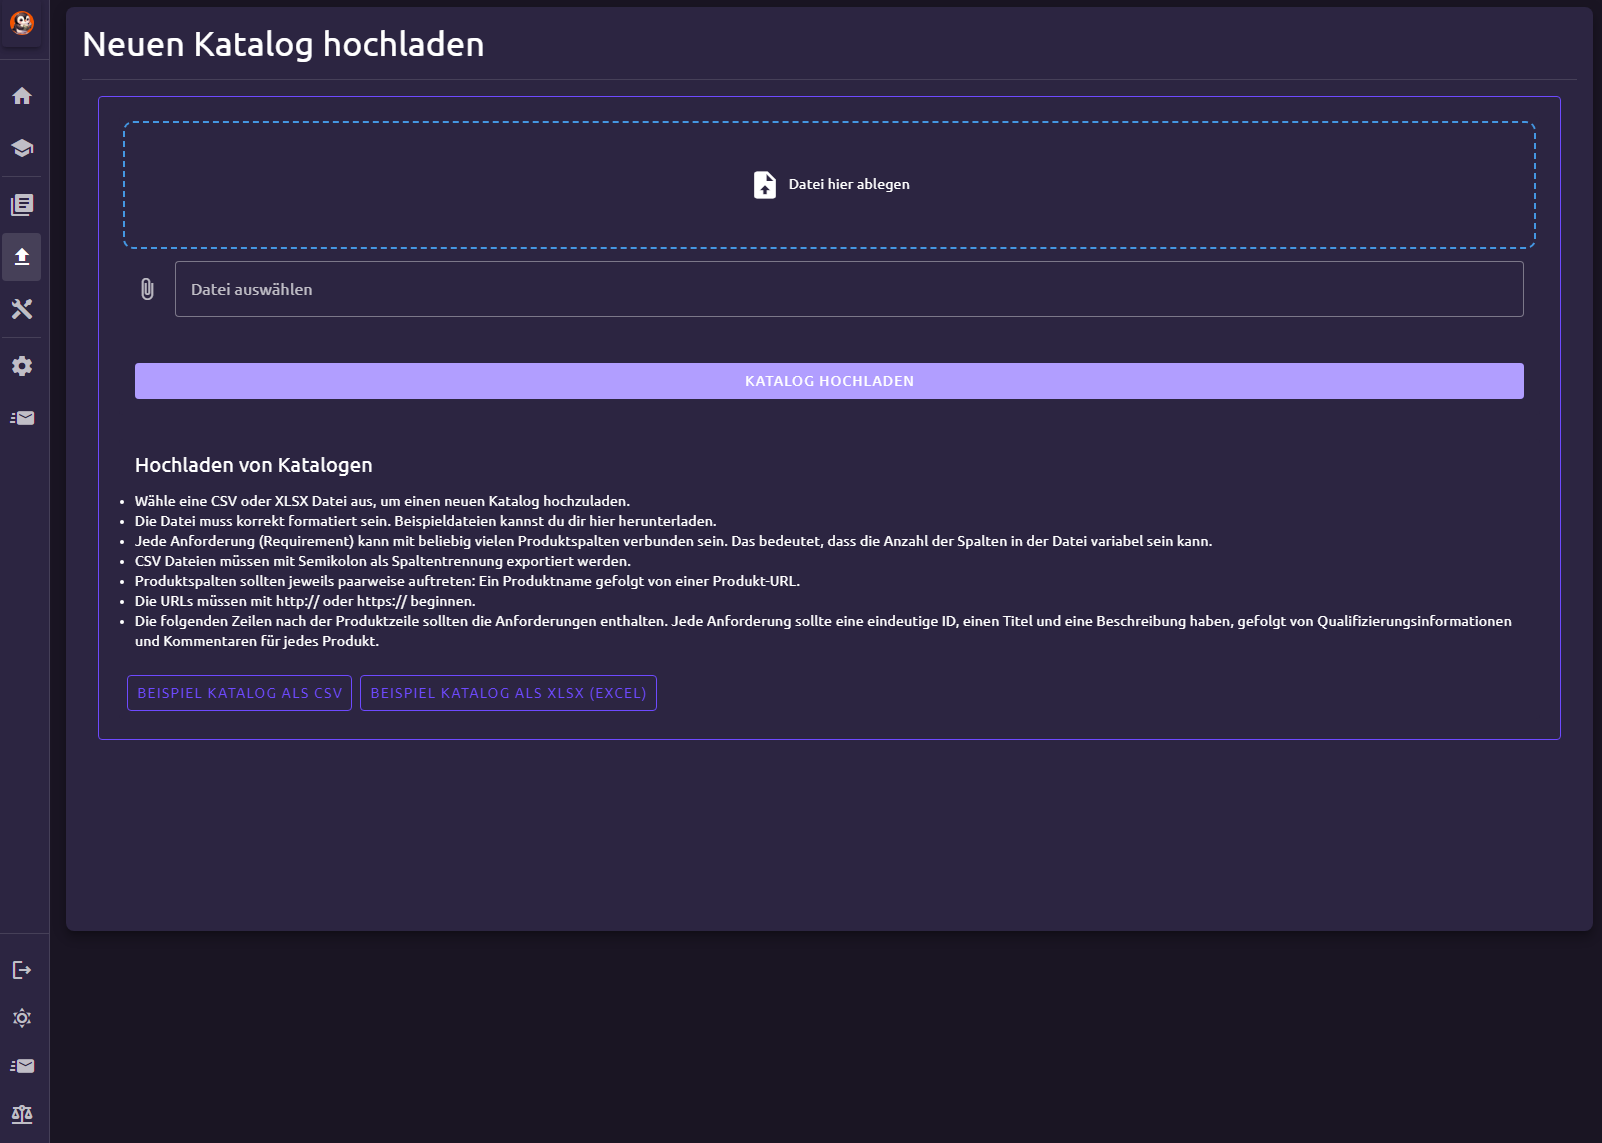
\includegraphics[width=1.0\textwidth]{assets/screenshots/finale_gui/Katalog_Upload.png}
    \caption{Hochladen eines Kataloges}
    \label{fig:catalog_upload_gui}
\end{figure}

\subsubsection{Lektionen}

Im weiteren werden die Lektionserstellung und die Lektionsbearbeitung genauer betrachtet. Lektionen sind zunächst frei und individuell erstellbar von Lehrenden. Ein Beispiel für eine solche Erstellung ist in der folgenden Grafik \ref{fig:lesson_create_gui} zu sehen. Es sind Titel, Beschreibungen und die Punktzahl anzugeben. Daraufhin liegt es daran, per Drag and Drop die Lektion mit verschiedenen Aufgaben zu füllen. In diesem Fall ist eine Aufgabe präsentiert, die darauf abzielt, Softwareprodukte zu einer aus einem Anforderungskatalog gewählten Anforderung zu evaluieren. 
Für die Lehrenden wird hierfür die Erstellung der Aufgabe erleichtert, indem die Anforderung direkt aus hochgeladenen Katalogen ausgewählt werden kann, zusammen mit allen zugehörigen Produkten und Bewertungen. 

\begin{figure}[H]
    \centering
    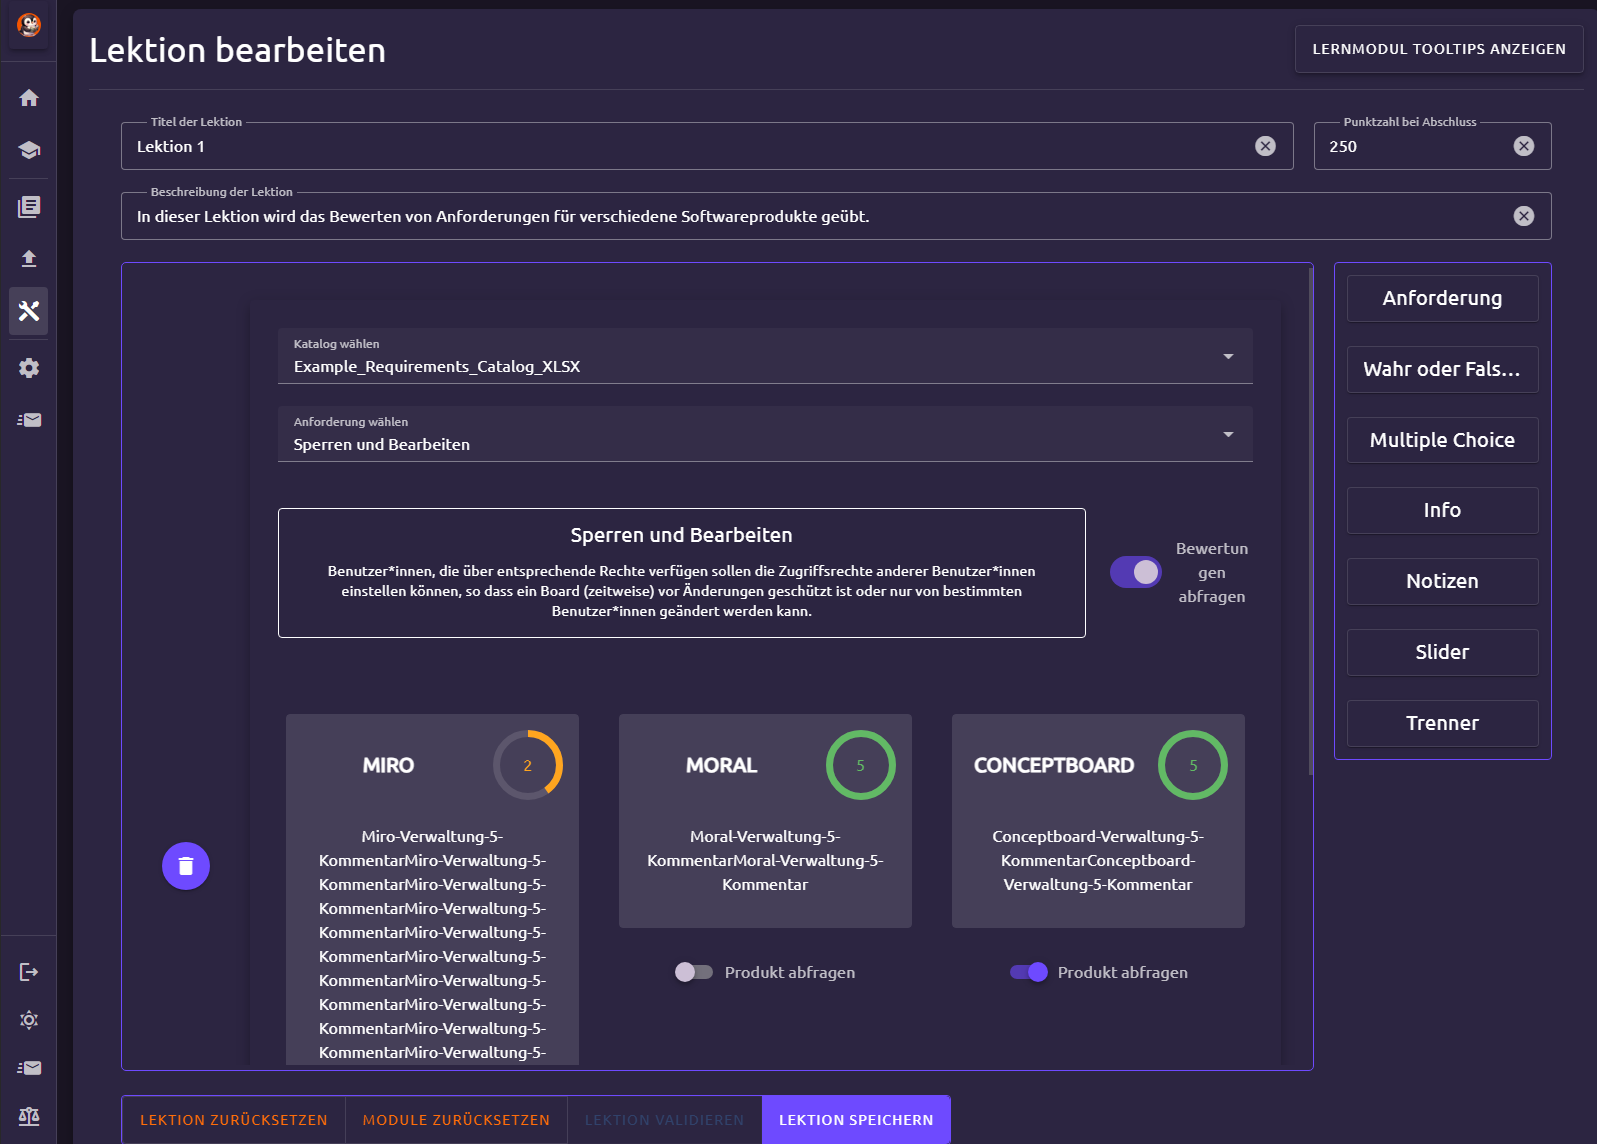
\includegraphics[width=1.0\textwidth]{assets/screenshots/finale_gui/Lektion_Erstellung_mit_Inhalt.png}
    \caption{Erstellung einer Lektion mit beispielhaften Inhalten}
    \label{fig:lesson_create_gui}
\end{figure}

Die abschließende Lektion kann dann veröffentlicht werden und wird somit zugänglich für Lernende. Diese können die Lektion dann bearbeiten. Die Ansicht hierfür ist in Abbildung \ref{fig:student_lesson_1_gui} präsentiert. Es werden auch hier wieder Unterschiede im Vergleich zu den zuvor präsentierten Mock-Ups deutlich, wie z.B. in \ref{fig:Software-Erprobung-1}. Einen Anforderungskatalog mit mehreren Reihen und Spalten an Daten in einer Lektion einzusetzen bietet einige Schwierigkeiten. Der Katalog würde sehr viel Platz einnehmen, je nach Anzahl der Anforderungen und zu bewertenden Produkte. Wenn zusätzlioch noch weitere Fragetypen und Komponenten verwendet werden, kann die Lektion schnell unübersichtlich und überwältigend wirken. Deshalb wird der Fokus nun, anstelle auf einen kompletten Kataloge, nur auf die zu bearbeitende Anforderung gesetzt. Es können weiterhin mehrere Anforderungen einzeln abgefragt werden, aber der Lernende geht hierbei Schritt für Schritt vor, anstatt direkt mit allen Anforderungen konfrontiert und möglicherweise eingeschüchtert zu werden. 

\begin{figure}[H]
    \centering
    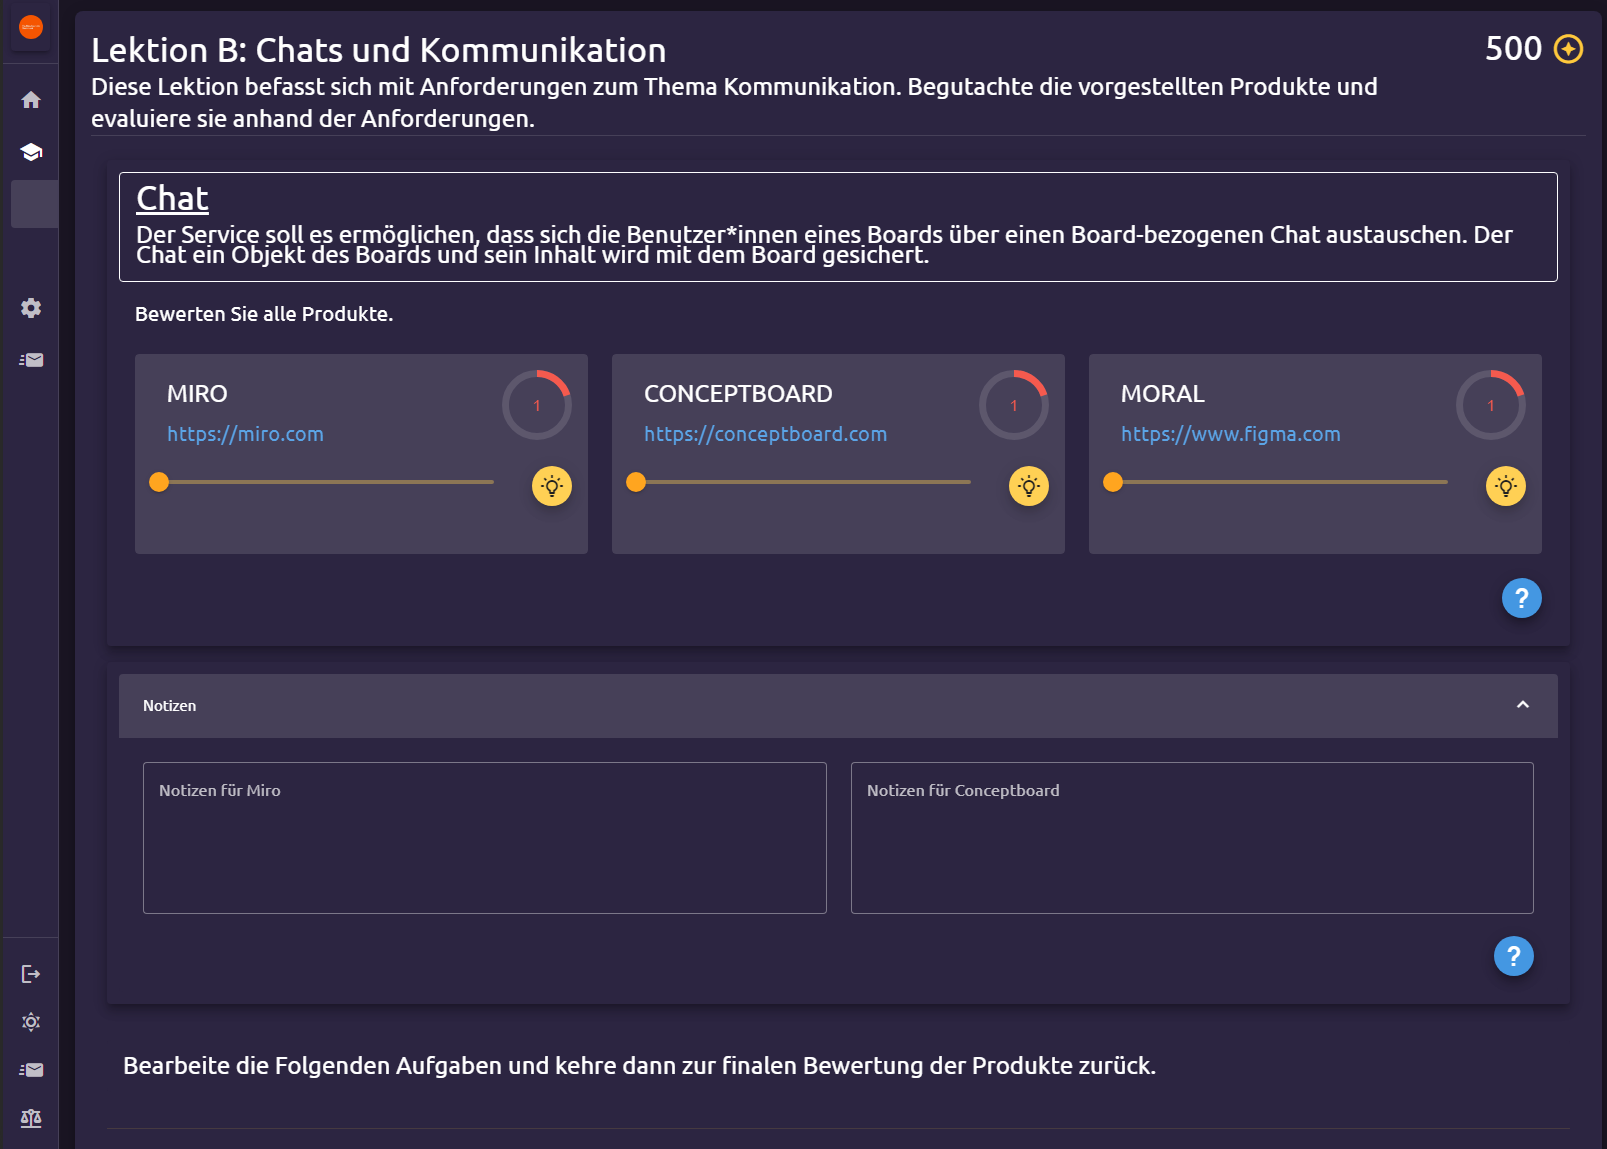
\includegraphics[width=1.0\textwidth]{assets/screenshots/finale_gui/Lektion_Lernende_1.png}
    \caption{Bearbeitung einer Lektion durch Lernende}
    \label{fig:student_lesson_1_gui}
\end{figure}

Es wird außerdem nicht mehr eine Tabelle dynamisch ausgefüllt, sondern interaktive Elemente genutzt. Für jedes Softwareprodukt kann ein Slider verwendet werden, welcher per Mausklick bewegt werden kann. Dadurch soll eine Qualifizierung des Produktes stattfinden. 
Die Idee der Notizen wurde hier weiterhin verfolgt. Sie können Lektionen an unterschiedlichen Stellen hinzugefügt werden, so dass Lernende ihre Gedanken festhalten können. Diese werden weiterhin nicht bewertet. 
Die traditionellen Herangehensweise der Evaluierung und Erprobung von Softwareprodukten mit Tabellen wird hier also etwas abgewandelt. Es wird auf spielerische Elemente und weniger Überflutung von Informationen gesetzt, um den Lernenden mehr Interaktion und Motivation zu ermöglichen.
       
\begin{itemize}
    \item Designentscheidungen
    \item Benachrichtigungen für Feedback
    \item Icons
    \item Themes
    \item Farben
    \item Responsivität
\end{itemize}
- große Änderungen und Gründe erläutern
- Layout für mehr Platz und weniger Ablenkungen
- Herausforderungen und Lösungen
- modernes ansprechendes Design (motivierend, nicht überfordernd)   
\section{Auswahl von grundlegenden Technologien}

- Enscheidungskriterien auflisten und erläutern: Skalierbarkeit, Leistung, Benutzerfreundlichkeit, Community-Support und Kosten


\subsection{Backend-as-a-Service}
- Erläuterung, warum sich für BaaS Lösung entscheiden wurde, z.B. schnelle Entwicklung, geringere Wartungskosten und Skalierbarkeit.
- Anforderungen die Erfüllt werden sollten: (Echtzeit)-Datenbank, Authentifizierung, Edge Functions, Open-Source-Natur, geringe Kosten usw.

\subsubsection{Firebase}
- Lead Solution von Google -> Starke Bindung an Google Ecosystem, Diskussion in Bezug auf Integration, Sicherheit und Verfügbarkeit
- Einfache integrastion von Google-Diensten (z.B. Google Analytics, Google Ads)
- Verwendung vertrauter Authentifizierungsmechanismen (z.B. Google Sign-In)
-> Wenig Flexibilität bei der Anpassung
-> Eigene DB Syntax...

\subsubsection{Supabase}
- Open Source alternative zu Firebase+, Vorteile beleuchten: Größere Flexibilität und Anpassungsmöglichkeiten, open Source Technologien, Optionen Services selbst zu hosten
- Community-getriebene Entwicklung
- SQL-Unterstützung, gut da viel mit Datenbank gearbeitet wird

\subsubsection{Fazit}
- Erläutern, warum sich für Supabase entschieden wurde, basierend auf den spezifischen Anforderungen und Zielen des Projekts

\subsection{Javascript Frontend Framework}

- Kurzer Vergleich Angular, Rect, Vue ->  Popularität, Leistungsfähigkeit, Lernkurve 
- Auf Projektspezifikationen beziehen ->  Guten Dokumentation, reaktivität,
- Bedeutung eines robusten Frontends und wie dies die Benutzererfahrung beeinflusst.

\subsubsection{UI Komponenten Bibliothek/Framework}
- Ersten Versuch mit Nuxt beschreiben und warum sich dagegen entschieden wurde.
- Vergleichene UI-Bibiotheken: Vuetify, Vuesax, Element, Vue Tailwind kurz erläutern und entscheidung begründen. Vergleich auf: Look'n'Feel, Ob noch unterstützt, Enthaltene Components(Darstellung von Daten, Profilbezogenen Elementen...), Support (Forum, Discord etc.), Kosten, 
- Integration beschreiben, wie Personalisiert?

\section{Projektmanagement,deployment und -planung}
- Einleitung

\subsection{Github}
- Wurde ohne großen Vergleich ausgewählt, da industry leading und Angebotene Funktionen wie Boards, Actions für Supabase und Deployment via Pages, Issue Tracking,

\subsubsection{Projects}
- Projektverwaltung. Zwar wurde Wasserfall Modell genutzt. Aber dennoch Elemente aus Agiler entwicklung wie Tasks und Storypoints zur Aufwandsschätzung übernommen, um übergang in Agiles Modell zu vereinfachen/unterstützen.

\subsubsection{Pages}
- Einfaches Deployment von Statischen Pages -> Hervorrgagen und Frontend Prototypen zu teilen

\subsubsection{Actions}
- Deploy Supabae Functions
- Deploy App
- Update DB Types

\section{Datenbankmodell}
- Diagramme und Erläuterungen
- Entscheidung, Jsons zu nutzen anstatt feingranulierte Tabellen für Lektionen und Fragetypen

\subsection{Tabelle catalogs}
\subsubsection{Tabelle requirements}
\subsubsection{Tabelle products}
\subsection{Tabelle lessons}
\subsection{Tabelle questions}
\subsection{Tabelle users}
\subsection{Tabelle profiles}
\subsection{Weitere Hilfstabellen}